\documentclass[10pt]{article}
% Names and product identity live in identity.tex. Preprint build: \anonfalse there.
% Review build: scripts/make_anon.py (anonymous identity.tex, \anontrue, [tmlr] without preprint).
% Camera-ready: [accepted].
% Everything in the manuscript that identifies the authors or their product.
% scripts/make_anon.py replaces this file with an anonymous version for review.
\newif\ifanon
\anonfalse
\newcommand{\product}{Kodama}        % the product, in running text
\newcommand{\promptname}{Kodama}     % the product name inside the quoted system prompt
\newcommand{\framework}{Circumstances}
\newcommand{\paperauthor}{\name Anton Chernov \email anton@aenimalabs.com \\
      \addr Aenima Labs}

\ifanon\usepackage{tmlr}\else\usepackage[preprint]{tmlr}\fi

\usepackage{amsmath,amssymb}
\usepackage{graphicx}
\usepackage{booktabs}
\usepackage{tabularx}
\usepackage{array}
\usepackage{enumitem}
\usepackage{float}
\usepackage{xcolor}
\usepackage{tikz}
\usetikzlibrary{arrows.meta,calc}
\usepackage[colorlinks=true,linkcolor=black,citecolor=black,urlcolor=black]{hyperref}
\usepackage{url}

% Generated by src/make_numbers.py. Do not edit.
\newcommand{\EoneTurns}{4,086}
\newcommand{\EoneSessions}{262}
\newcommand{\EoneMemMedian}{296}
\newcommand{\EoneMemMin}{16}
\newcommand{\EoneMemMax}{665}
\newcommand{\EoneWordsMean}{21}
\newcommand{\OvLone}{0.50}
\newcommand{\OvLoneCI}{[0.49, 0.51]}
\newcommand{\OvLtwo}{0.32}
\newcommand{\OvLtwoCI}{[0.31, 0.33]}
\newcommand{\OvLthree}{0.18}
\newcommand{\OvLthreeCI}{[0.17, 0.19]}
\newcommand{\OvLsix}{0.12}
\newcommand{\OvLsixCI}{[0.11, 0.13]}
\newcommand{\OvRand}{0.08}
\newcommand{\OvRandCI}{[0.07, 0.09]}
\newcommand{\OvPquarter}{0.71}
\newcommand{\OvPquarterCI}{[0.70, 0.72]}
\newcommand{\OvPhalf}{0.77}
\newcommand{\OvPhalfCI}{[0.76, 0.78]}
\newcommand{\OvPthreeq}{0.85}
\newcommand{\OvPthreeqCI}{[0.84, 0.85]}
\newcommand{\OvWoneLone}{0.14}
\newcommand{\OvWonePhalf}{0.49}
\newcommand{\OvWfiveLone}{0.62}
\newcommand{\OvWfivePhalf}{0.83}
\newcommand{\TopOneLone}{69}
\newcommand{\TopOnePhalf}{92}
\newcommand{\ShiftLoneQone}{0.53}
\newcommand{\ShiftLoneQfour}{0.48}
\newcommand{\ShiftPhalfQone}{0.77}
\newcommand{\ShiftPhalfQfour}{0.79}
\newcommand{\HindTurns}{3,824}
\newcommand{\HindFresh}{0.152}
\newcommand{\HindFreshCI}{[0.142, 0.163]}
\newcommand{\HindLone}{0.134}
\newcommand{\HindLoneCI}{[0.123, 0.146]}
\newcommand{\HindLthree}{0.105}
\newcommand{\HindLthreeCI}{[0.098, 0.113]}
\newcommand{\HindPhalf}{0.137}
\newcommand{\HindPhalfCI}{[0.128, 0.147]}
\newcommand{\HindRand}{0.066}
\newcommand{\HindRandCI}{[0.060, 0.074]}
\newcommand{\HindRetained}{79}
\newcommand{\UttMedianSec}{7.2}
\newcommand{\SlackMedianSec}{16}
\newcommand{\TimTurnFive}{0.49}
\newcommand{\TimTurnTwelve}{0.41}
\newcommand{\TimTurnTwentySeven}{0.20}
\newcommand{\TimStreamTenth}{0.85}
\newcommand{\TimStreamOne}{0.82}
\newcommand{\TimStreamTwo}{0.76}
\newcommand{\TimStreamFive}{0.59}
\newcommand{\TimStreamOneFast}{0.79}
\newcommand{\TimTurnTwelveFast}{0.32}
\newcommand{\EtwoTrials}{1,200}
\newcommand{\RecNone}{0}
\newcommand{\RecNoneCI}{[0, 0]}
\newcommand{\GoldNone}{0}
\newcommand{\AbstNone}{100}
\newcommand{\SrchNone}{0}
\newcommand{\ContNone}{0}
\newcommand{\ShiftNone}{0}
\newcommand{\UnpNone}{0}
\newcommand{\StatedNone}{0}
\newcommand{\DeclinedNone}{98}
\newcommand{\OtherNone}{2}
\newcommand{\RecTool}{82}
\newcommand{\RecToolCI}{[71, 91]}
\newcommand{\GoldTool}{85}
\newcommand{\AbstTool}{84}
\newcommand{\SrchTool}{98}
\newcommand{\ContTool}{80}
\newcommand{\ShiftTool}{92}
\newcommand{\UnpTool}{74}
\newcommand{\StatedTool}{86}
\newcommand{\DeclinedTool}{14}
\newcommand{\OtherTool}{0}
\newcommand{\RecBlock}{75}
\newcommand{\RecBlockCI}{[59, 89]}
\newcommand{\GoldBlock}{83}
\newcommand{\AbstBlock}{90}
\newcommand{\SrchBlock}{0}
\newcommand{\ContBlock}{62}
\newcommand{\ShiftBlock}{68}
\newcommand{\UnpBlock}{94}
\newcommand{\StatedBlock}{65}
\newcommand{\DeclinedBlock}{30}
\newcommand{\OtherBlock}{5}
\newcommand{\RecLag}{19}
\newcommand{\RecLagCI}{[7, 33]}
\newcommand{\GoldLag}{23}
\newcommand{\AbstLag}{90}
\newcommand{\SrchLag}{0}
\newcommand{\ContLag}{24}
\newcommand{\ShiftLag}{0}
\newcommand{\UnpLag}{34}
\newcommand{\StatedLag}{12}
\newcommand{\DeclinedLag}{88}
\newcommand{\OtherLag}{0}
\newcommand{\RecPre}{43}
\newcommand{\RecPreCI}{[27, 60]}
\newcommand{\GoldPre}{50}
\newcommand{\AbstPre}{94}
\newcommand{\SrchPre}{0}
\newcommand{\ContPre}{34}
\newcommand{\ShiftPre}{34}
\newcommand{\UnpPre}{62}
\newcommand{\StatedPre}{34}
\newcommand{\DeclinedPre}{66}
\newcommand{\OtherPre}{0}
\newcommand{\RecHyb}{43}
\newcommand{\RecHybCI}{[29, 57]}
\newcommand{\GoldHyb}{47}
\newcommand{\AbstHyb}{90}
\newcommand{\SrchHyb}{40}
\newcommand{\ContHyb}{66}
\newcommand{\ShiftHyb}{20}
\newcommand{\UnpHyb}{42}
\newcommand{\StatedHyb}{43}
\newcommand{\DeclinedHyb}{57}
\newcommand{\OtherHyb}{0}
\newcommand{\DiffBlockLag}{55}
\newcommand{\DiffBlockLagCI}{[37, 73]}
\newcommand{\DiffBlockPre}{31}
\newcommand{\DiffBlockPreCI}{[15, 48]}
\newcommand{\DiffBlockTool}{$-$7}
\newcommand{\DiffBlockToolCI}{[$-$24, 8]}
\newcommand{\DiffPreLag}{24}
\newcommand{\DiffPreLagCI}{[10, 39]}
\newcommand{\DiffHybLag}{23}
\newcommand{\DiffHybLagCI}{[12, 36]}
\newcommand{\DiffBlockHyb}{32}
\newcommand{\DiffBlockHybCI}{[14, 49]}
\newcommand{\DiffToolLag}{63}
\newcommand{\DiffToolLagCI}{[46, 78]}
\newcommand{\PassGivenGold}{91}
\newcommand{\PassGivenGoldN}{433}
\newcommand{\PassGivenNoGoldN}{317}
\newcommand{\PreBlockMed}{15}
\newcommand{\PreBlockPninety}{17}
\newcommand{\PreToolMed}{426}
\newcommand{\PreToolPninety}{820}
\newcommand{\PreHybMed}{364}
\newcommand{\PreHybPninety}{1137}
\newcommand{\OffpathMed}{14}
\newcommand{\RepairedHyb}{51}
\newcommand{\RepairedTool}{1}
\newcommand{\FormatErrors}{1}
\newcommand{\RunErrors}{0}
\newcommand{\SrchShiftTool}{94}
\newcommand{\SrchShiftHyb}{20}
\newcommand{\SrchUnpTool}{100}
\newcommand{\SrchUnpHyb}{10}
\newcommand{\SrchContHyb}{82}
\newcommand{\ThTrials}{1,200}
\newcommand{\ThRecNone}{0}
\newcommand{\ThRecNoneCI}{[0, 0]}
\newcommand{\ThGoldNone}{0}
\newcommand{\ThAbstNone}{100}
\newcommand{\ThDeclinedNone}{100}
\newcommand{\ThOtherNone}{0}
\newcommand{\ThContNone}{0}
\newcommand{\ThShiftNone}{0}
\newcommand{\ThUnpNone}{0}
\newcommand{\ThReplyNone}{4.7}
\newcommand{\ThRecTool}{85}
\newcommand{\ThRecToolCI}{[75, 94]}
\newcommand{\ThGoldTool}{86}
\newcommand{\ThAbstTool}{96}
\newcommand{\ThDeclinedTool}{15}
\newcommand{\ThOtherTool}{0}
\newcommand{\ThContTool}{72}
\newcommand{\ThShiftTool}{98}
\newcommand{\ThUnpTool}{86}
\newcommand{\ThReplyTool}{9.2}
\newcommand{\ThRecBlock}{77}
\newcommand{\ThRecBlockCI}{[63, 90]}
\newcommand{\ThGoldBlock}{83}
\newcommand{\ThAbstBlock}{98}
\newcommand{\ThDeclinedBlock}{26}
\newcommand{\ThOtherBlock}{5}
\newcommand{\ThContBlock}{66}
\newcommand{\ThShiftBlock}{72}
\newcommand{\ThUnpBlock}{94}
\newcommand{\ThRecLag}{21}
\newcommand{\ThRecLagCI}{[8, 36]}
\newcommand{\ThGoldLag}{23}
\newcommand{\ThAbstLag}{98}
\newcommand{\ThDeclinedLag}{85}
\newcommand{\ThOtherLag}{0}
\newcommand{\ThContLag}{30}
\newcommand{\ThShiftLag}{0}
\newcommand{\ThUnpLag}{34}
\newcommand{\ThReplyLag}{6.2}
\newcommand{\ThRecPre}{48}
\newcommand{\ThRecPreCI}{[30, 65]}
\newcommand{\ThGoldPre}{50}
\newcommand{\ThAbstPre}{98}
\newcommand{\ThDeclinedPre}{60}
\newcommand{\ThOtherPre}{0}
\newcommand{\ThContPre}{40}
\newcommand{\ThShiftPre}{40}
\newcommand{\ThUnpPre}{64}
\newcommand{\ThReplyPre}{6.0}
\newcommand{\ThRecHyb}{87}
\newcommand{\ThRecHybCI}{[78, 95]}
\newcommand{\ThGoldHyb}{89}
\newcommand{\ThAbstHyb}{94}
\newcommand{\ThDeclinedHyb}{6}
\newcommand{\ThOtherHyb}{0}
\newcommand{\ThContHyb}{88}
\newcommand{\ThShiftHyb}{100}
\newcommand{\ThUnpHyb}{74}
\newcommand{\ThReplyHyb}{11.3}
\newcommand{\ThDiffBlockLag}{56}
\newcommand{\ThDiffBlockLagCI}{[37, 74]}
\newcommand{\ThDiffBlockTool}{$-$8}
\newcommand{\ThDiffBlockToolCI}{[$-$23, 7]}
\newcommand{\ThDiffPreLag}{27}
\newcommand{\ThDiffPreLagCI}{[10, 43]}
\newcommand{\ThDiffBlockHyb}{$-$10}
\newcommand{\ThDiffBlockHybCI}{[$-$27, 7]}
\newcommand{\ThDiffHybLag}{66}
\newcommand{\ThDiffHybLagCI}{[51, 79]}
\newcommand{\ThPassGivenGold}{96}
\newcommand{\ThPassGivenGoldN}{497}
\newcommand{\ThPassGivenNoGold}{0}
\newcommand{\ThPassGivenNoGoldN}{253}
\newcommand{\ThPassedNoGold}{0}
\newcommand{\ThSrchShiftHyb}{100}
\newcommand{\ThSrchUnpHyb}{84}
\newcommand{\ThSrchContHyb}{94}
\newcommand{\ThSrchUnpTool}{100}
\newcommand{\ThSrchHyb}{94}
\newcommand{\ThSrchTool}{100}
\newcommand{\ThRepairedHyb}{6}
\newcommand{\ThRepairedTool}{0}
\newcommand{\ThFormatErrors}{0}
\newcommand{\ThRunErrors}{0}
\newcommand{\ThPreHybMed}{5.6}
\newcommand{\ThPreToolMed}{2.0}
\newcommand{\QwTrials}{1,200}
\newcommand{\QwRecNone}{0}
\newcommand{\QwRecNoneCI}{[0, 0]}
\newcommand{\QwGoldNone}{0}
\newcommand{\QwAbstNone}{56}
\newcommand{\QwDeclinedNone}{30}
\newcommand{\QwOtherNone}{70}
\newcommand{\QwContNone}{0}
\newcommand{\QwShiftNone}{0}
\newcommand{\QwUnpNone}{0}
\newcommand{\QwReplyNone}{0.7}
\newcommand{\QwRecTool}{67}
\newcommand{\QwRecToolCI}{[51, 83]}
\newcommand{\QwGoldTool}{67}
\newcommand{\QwAbstTool}{44}
\newcommand{\QwDeclinedTool}{2}
\newcommand{\QwOtherTool}{2}
\newcommand{\QwContTool}{92}
\newcommand{\QwShiftTool}{100}
\newcommand{\QwUnpTool}{10}
\newcommand{\QwReplyTool}{1.5}
\newcommand{\QwRecBlock}{80}
\newcommand{\QwRecBlockCI}{[65, 92]}
\newcommand{\QwGoldBlock}{83}
\newcommand{\QwAbstBlock}{48}
\newcommand{\QwDeclinedBlock}{13}
\newcommand{\QwOtherBlock}{12}
\newcommand{\QwContBlock}{70}
\newcommand{\QwShiftBlock}{80}
\newcommand{\QwUnpBlock}{90}
\newcommand{\QwReplyBlock}{0.8}
\newcommand{\QwRecLag}{23}
\newcommand{\QwRecLagCI}{[10, 40]}
\newcommand{\QwGoldLag}{23}
\newcommand{\QwAbstLag}{72}
\newcommand{\QwDeclinedLag}{68}
\newcommand{\QwOtherLag}{17}
\newcommand{\QwContLag}{30}
\newcommand{\QwShiftLag}{0}
\newcommand{\QwUnpLag}{40}
\newcommand{\QwReplyLag}{0.7}
\newcommand{\QwRecPre}{49}
\newcommand{\QwRecPreCI}{[31, 67]}
\newcommand{\QwGoldPre}{50}
\newcommand{\QwAbstPre}{72}
\newcommand{\QwDeclinedPre}{45}
\newcommand{\QwOtherPre}{15}
\newcommand{\QwContPre}{40}
\newcommand{\QwShiftPre}{40}
\newcommand{\QwUnpPre}{66}
\newcommand{\QwReplyPre}{0.8}
\newcommand{\QwRecHyb}{37}
\newcommand{\QwRecHybCI}{[21, 53]}
\newcommand{\QwGoldHyb}{37}
\newcommand{\QwAbstHyb}{76}
\newcommand{\QwDeclinedHyb}{59}
\newcommand{\QwOtherHyb}{5}
\newcommand{\QwContHyb}{40}
\newcommand{\QwShiftHyb}{32}
\newcommand{\QwUnpHyb}{38}
\newcommand{\QwReplyHyb}{1.2}
\newcommand{\QwDiffBlockLag}{57}
\newcommand{\QwDiffBlockLagCI}{[39, 74]}
\newcommand{\QwDiffBlockTool}{13}
\newcommand{\QwDiffBlockToolCI}{[$-$9, 34]}
\newcommand{\QwDiffPreLag}{25}
\newcommand{\QwDiffPreLagCI}{[10, 41]}
\newcommand{\QwDiffBlockHyb}{43}
\newcommand{\QwDiffBlockHybCI}{[26, 61]}
\newcommand{\QwDiffHybLag}{13}
\newcommand{\QwDiffHybLagCI}{[3, 26]}
\newcommand{\QwPassGivenGold}{98}
\newcommand{\QwPassGivenGoldN}{392}
\newcommand{\QwPassGivenNoGold}{0}
\newcommand{\QwPassGivenNoGoldN}{358}
\newcommand{\QwPassedNoGold}{0}
\newcommand{\QwSrchShiftHyb}{32}
\newcommand{\QwSrchUnpHyb}{4}
\newcommand{\QwSrchContHyb}{30}
\newcommand{\QwSrchUnpTool}{12}
\newcommand{\QwSrchHyb}{22}
\newcommand{\QwSrchTool}{78}
\newcommand{\QwRepairedHyb}{59}
\newcommand{\QwRepairedTool}{44}
\newcommand{\QwFormatErrors}{0}
\newcommand{\QwRunErrors}{0}
\newcommand{\QwPreHybMed}{0.5}
\newcommand{\QwPreToolMed}{0.6}
\newcommand{\ReplyNone}{0.4}
\newcommand{\ReplyTool}{1.4}
\newcommand{\ReplyBlock}{0.8}
\newcommand{\ReplyLag}{0.5}
\newcommand{\ReplyPre}{0.6}
\newcommand{\ReplyHyb}{1.3}
\newcommand{\AllNoGoldN}{928}
\newcommand{\AllNoGoldPassed}{0}
\newcommand{\AllTrials}{3,600}
\newcommand{\KTrials}{1,000}
\newcommand{\KErrors}{0}
\newcommand{\KTemplated}{61}
\newcommand{\KfTemplated}{215}
\newcommand{\KRecTool}{63}
\newcommand{\KRecToolCI}{[49, 78]}
\newcommand{\KGoldTool}{0}
\newcommand{\KSrchTool}{78}
\newcommand{\KPathTool}{6.1}
\newcommand{\KAbstToolTool}{32}
\newcommand{\KAbstWordsTool}{36}
\newcommand{\KContTool}{88}
\newcommand{\KShiftTool}{92}
\newcommand{\KUnpTool}{10}
\newcommand{\KfRecTool}{59}
\newcommand{\KfTmplTool}{15}
\newcommand{\KRecLag}{29}
\newcommand{\KRecLagCI}{[13, 45]}
\newcommand{\KGoldLag}{33}
\newcommand{\KSrchLag}{0}
\newcommand{\KPathLag}{3.6}
\newcommand{\KAbstToolLag}{12}
\newcommand{\KAbstWordsLag}{74}
\newcommand{\KContLag}{50}
\newcommand{\KShiftLag}{0}
\newcommand{\KUnpLag}{36}
\newcommand{\KfRecLag}{13}
\newcommand{\KfTmplLag}{46}
\newcommand{\KRecBlock}{84}
\newcommand{\KRecBlockCI}{[71, 95]}
\newcommand{\KGoldBlock}{93}
\newcommand{\KSrchBlock}{0}
\newcommand{\KPathBlock}{4.1}
\newcommand{\KAbstToolBlock}{12}
\newcommand{\KAbstWordsBlock}{64}
\newcommand{\KContBlock}{78}
\newcommand{\KShiftBlock}{100}
\newcommand{\KUnpBlock}{74}
\newcommand{\KfRecBlock}{43}
\newcommand{\KfTmplBlock}{59}
\newcommand{\KRecBoth}{85}
\newcommand{\KRecBothCI}{[72, 95]}
\newcommand{\KGoldBoth}{95}
\newcommand{\KSrchBoth}{0}
\newcommand{\KPathBoth}{4.2}
\newcommand{\KAbstToolBoth}{14}
\newcommand{\KAbstWordsBoth}{72}
\newcommand{\KContBoth}{84}
\newcommand{\KShiftBoth}{98}
\newcommand{\KUnpBoth}{72}
\newcommand{\KfRecBoth}{37}
\newcommand{\KfTmplBoth}{72}
\newcommand{\KRecHyb}{67}
\newcommand{\KRecHybCI}{[51, 82]}
\newcommand{\KGoldHyb}{33}
\newcommand{\KSrchHyb}{80}
\newcommand{\KPathHyb}{6.3}
\newcommand{\KAbstToolHyb}{30}
\newcommand{\KAbstWordsHyb}{58}
\newcommand{\KContHyb}{98}
\newcommand{\KShiftHyb}{80}
\newcommand{\KUnpHyb}{22}
\newcommand{\KfRecHyb}{59}
\newcommand{\KfTmplHyb}{23}
\newcommand{\KDiffBlockLag}{55}
\newcommand{\KDiffBlockLagCI}{[36, 74]}
\newcommand{\KDiffBlockTool}{21}
\newcommand{\KDiffBlockToolCI}{[5, 37]}
\newcommand{\KDiffBothBlock}{1}
\newcommand{\KDiffBothBlockCI}{[$-$6, 6]}
\newcommand{\KDiffHybTool}{3}
\newcommand{\KDiffHybToolCI}{[$-$9, 15]}
\newcommand{\KGuessMin}{12}
\newcommand{\KGuessMax}{50}
\newcommand{\KPassGivenGold}{89}
\newcommand{\KPassGivenGoldN}{332}
\newcommand{\KNoGoldN}{118}
\newcommand{\KNoGoldPassed}{0}
\newcommand{\KBlockMs}{97}
\newcommand{\KOffpathMs}{19}
\newcommand{\KLlmTool}{3.9}
\newcommand{\KLlmBlock}{1.7}

% Diagram figures (TikZ). Colours match the data figures.
\definecolor{ink}{HTML}{1A1A19}
\definecolor{muted}{HTML}{5F5E5A}
\definecolor{hair}{HTML}{C3C2B7}
\definecolor{speech}{HTML}{EEEDE8}
\definecolor{gen}{HTML}{CDE2FB}
\definecolor{rec}{HTML}{F9D5C6}
\definecolor{blue}{HTML}{2A78D6}
\definecolor{orange}{HTML}{EB6834}

\newcommand{\tlbox}[5][]{% [style] x0 x1 y label
  \draw[draw=hair, line width=0.4pt, rounded corners=1.2pt, #1]
    (#2,#4-0.26) rectangle (#3,#4+0.26);
  \node[font=\scriptsize, text=ink] at ({(#2+#3)/2},#4) {#5};
}

\newcommand{\timelinefigure}{%
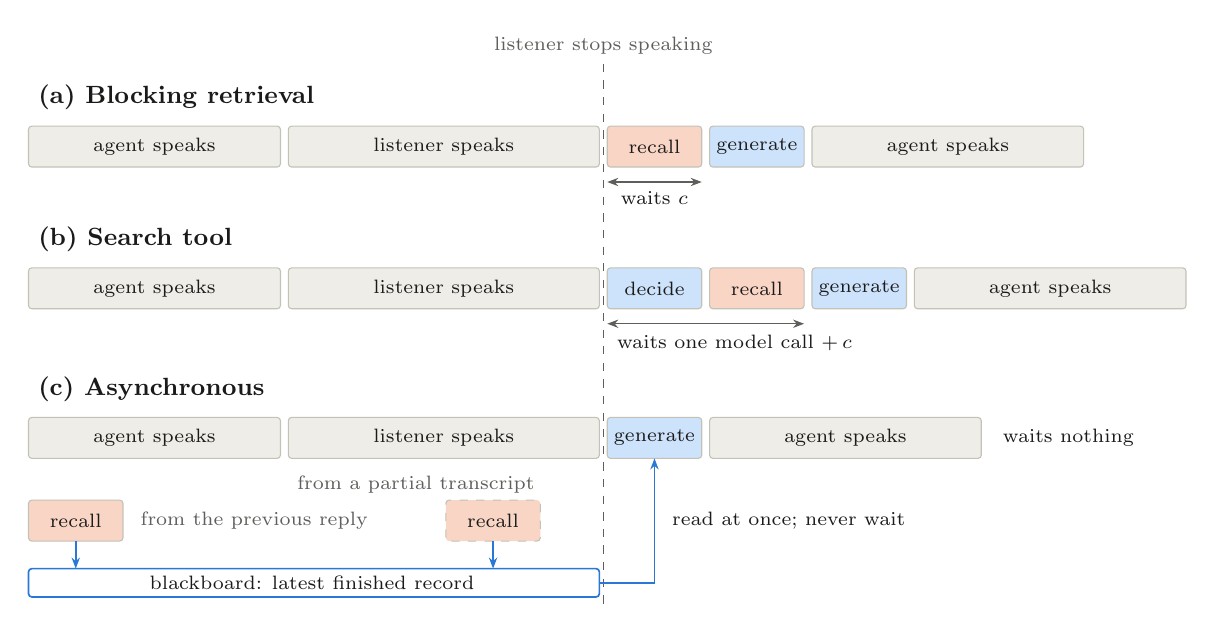
\begin{tikzpicture}[x=1cm, y=1cm, >={Stealth[length=4pt]}]
  % end of the listener's utterance
  \draw[muted, dashed, line width=0.5pt] (7.3,1.05) -- (7.3,-5.85);
  \node[font=\scriptsize, text=muted, anchor=south] at (7.3,1.05) {listener stops speaking};

  % (a) blocking
  \node[font=\small\bfseries, anchor=west, text=ink] at (0,0.62) {(a) Blocking retrieval};
  \tlbox[fill=speech]{0}{3.2}{0}{agent speaks}
  \tlbox[fill=speech]{3.3}{7.25}{0}{listener speaks}
  \tlbox[fill=rec]{7.35}{8.55}{0}{recall}
  \tlbox[fill=gen]{8.65}{9.85}{0}{generate}
  \tlbox[fill=speech]{9.95}{13.4}{0}{agent speaks}
  \draw[<->, muted, line width=0.5pt] (7.35,-0.45) -- node[below, font=\scriptsize, text=ink] {waits $c$} (8.55,-0.45);

  % (b) search tool
  \node[font=\small\bfseries, anchor=west, text=ink] at (0,-1.18) {(b) Search tool};
  \tlbox[fill=speech]{0}{3.2}{-1.8}{agent speaks}
  \tlbox[fill=speech]{3.3}{7.25}{-1.8}{listener speaks}
  \tlbox[fill=gen]{7.35}{8.55}{-1.8}{decide}
  \tlbox[fill=rec]{8.65}{9.85}{-1.8}{recall}
  \tlbox[fill=gen]{9.95}{11.15}{-1.8}{generate}
  \tlbox[fill=speech]{11.25}{14.7}{-1.8}{agent speaks}
  \draw[<->, muted, line width=0.5pt] (7.35,-2.25) -- (9.85,-2.25);
  \node[font=\scriptsize, text=ink, anchor=north west] at (7.35,-2.27) {waits one model call $+\,c$};

  % (c) asynchronous
  \node[font=\small\bfseries, anchor=west, text=ink] at (0,-3.08) {(c) Asynchronous};
  \tlbox[fill=speech]{0}{3.2}{-3.7}{agent speaks}
  \tlbox[fill=speech]{3.3}{7.25}{-3.7}{listener speaks}
  \tlbox[fill=gen]{7.35}{8.55}{-3.7}{generate}
  \tlbox[fill=speech]{8.65}{12.1}{-3.7}{agent speaks}
  \node[font=\scriptsize, text=ink, anchor=west] at (12.25,-3.7) {waits nothing};
  % background jobs
  \tlbox[fill=rec]{0}{1.2}{-4.75}{recall}
  \tlbox[fill=rec, dashed]{5.3}{6.5}{-4.75}{recall}
  \node[font=\scriptsize, text=muted, anchor=west] at (1.3,-4.75) {from the previous reply};
  \node[font=\scriptsize, text=muted, anchor=east] at (6.55,-4.3) {from a partial transcript};
  % blackboard
  \draw[draw=blue, fill=white, line width=0.6pt, rounded corners=1.2pt] (0,-5.72) rectangle (7.25,-5.36);
  \node[font=\scriptsize, text=ink] at (3.6,-5.54) {blackboard: latest finished record};
  \draw[->, blue, line width=0.6pt] (0.6,-5.01) -- (0.6,-5.36);
  \draw[->, blue, line width=0.6pt] (5.9,-5.01) -- (5.9,-5.36);
  \draw[->, blue, line width=0.6pt] (7.25,-5.54) -- (7.95,-5.54) -- (7.95,-3.96);
  \node[font=\scriptsize, text=ink, anchor=west] at (8.05,-4.75) {read at once; never wait};
\end{tikzpicture}}

\newcommand{\architecturefigure}{%
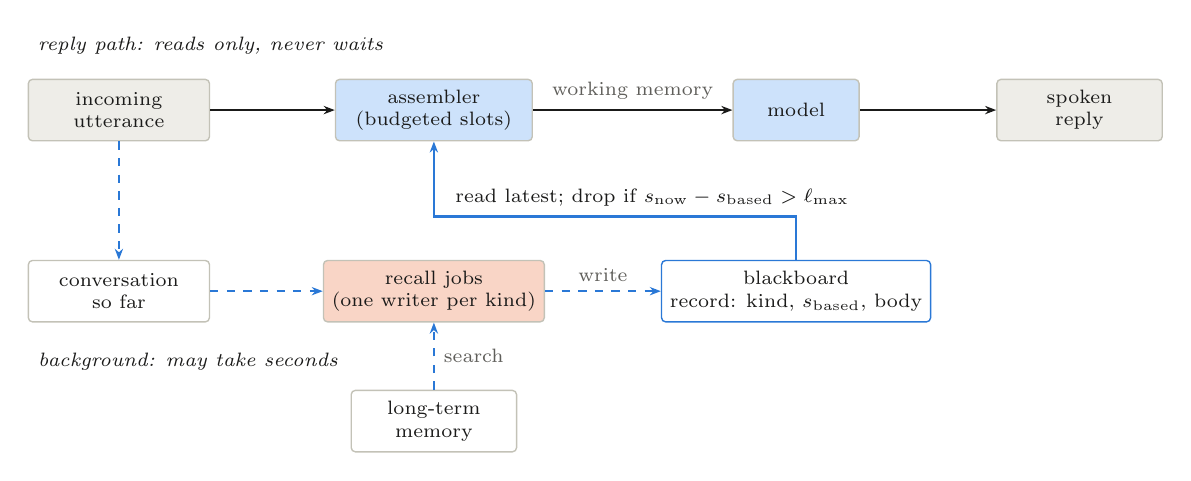
\begin{tikzpicture}[x=1cm, y=1cm, >={Stealth[length=4pt]},
    box/.style={draw=hair, line width=0.5pt, rounded corners=1.5pt, fill=white,
                align=center, font=\scriptsize, text=ink, minimum height=0.78cm, inner sep=3pt},
    fast/.style={->, ink, line width=0.9pt},
    slow/.style={->, blue, line width=0.6pt, dashed}]
  % fast path
  \node[box, fill=speech, minimum width=2.3cm] (utt) at (0,0) {incoming\\utterance};
  \node[box, fill=gen, minimum width=2.5cm] (asm) at (4.0,0) {assembler\\(budgeted slots)};
  \node[box, fill=gen, minimum width=1.6cm] (llm) at (8.6,0) {model};
  \node[box, fill=speech, minimum width=2.1cm] (rep) at (12.2,0) {spoken\\reply};
  \draw[fast] (utt) -- (asm);
  \draw[fast] (asm) -- node[above, font=\scriptsize, text=muted] {working memory} (llm);
  \draw[fast] (llm) -- (rep);
  \node[font=\scriptsize\itshape, text=ink, anchor=west] at (-1.15,0.82) {reply path: reads only, never waits};
  % slow path
  \node[box, minimum width=2.3cm] (evt) at (0,-2.3) {conversation\\so far};
  \node[box, fill=rec, minimum width=2.5cm] (bt) at (4.0,-2.3) {recall jobs\\(one writer per kind)};
  \node[box, draw=blue, minimum width=3.3cm] (bb) at (8.6,-2.3) {blackboard\\record: kind, $s_{\mathrm{based}}$, body};
  \node[box, minimum width=2.1cm] (mem) at (4.0,-3.95) {long-term\\memory};
  \draw[slow] (utt) -- (evt);
  \draw[slow] (evt) -- (bt);
  \draw[slow] (bt) -- node[above, font=\scriptsize, text=muted] {write} (bb);
  \draw[slow] (mem) -- node[right, font=\scriptsize, text=muted] {search} (bt);
  \draw[fast, blue] (bb.north) -- ++(0,0.55) -| (asm.south);
  \node[font=\scriptsize, text=ink, anchor=south west] at (4.15,-1.34)
       {read latest; drop if $s_{\mathrm{now}}-s_{\mathrm{based}}>\ell_{\max}$};
  \node[font=\scriptsize\itshape, text=ink, anchor=west] at (-1.15,-3.2) {background: may take seconds};
\end{tikzpicture}}

\graphicspath{{../figures/}}
\newcolumntype{Y}{>{\raggedright\arraybackslash}X}
\newcommand{\lmax}{\ell_{\max}}
\makeatletter\newcommand{\tabinput}[1]{\@@input #1 }\makeatother % expandable \input for table bodies

\title{Stale but on Time: What Asynchronous Memory Recall\\Costs a Real-Time Conversational Agent}

\author{\paperauthor}

\def\month{11}
\def\year{2026}
\def\openreview{\url{https://openreview.net/forum?id=XXXX}}

\begin{document}

\maketitle

\begin{abstract}
A voice agent has to reply quickly, and retrieving long-term memories on the reply path takes time. A common remedy moves recall off that path: background jobs prepare context, and the reply uses whatever is ready. The price is staleness, because the context was computed before the listener's latest words. We measure that price. Replaying \EoneTurns{} utterances from LoCoMo, a recall result computed one utterance early shares \OvLone{} of its top-5 memories with fresh retrieval; three utterances early it shares \OvLthree{}, close to the \OvRand{} obtained from unrelated context. Starting recall on a partial transcript recovers much of the loss (\OvPhalf{} at half the utterance). In \EtwoTrials{} end-to-end trials with a small local model, never-wait recall passes \RecLag\% of recall cases, against \RecBlock\% for blocking retrieval and \RecTool\% for a search tool; half-utterance prefetch reaches \RecPre\%. The misses are abstentions, not fabrications, and success depended entirely on whether the right memory was in context. Loading stale memories also made the model search less. Asynchronous recall should therefore carry only work that is too slow to block on, start on partial transcripts, and expire within one exchange.
\end{abstract}

\begingroup
\renewcommand\thefootnote{}\footnotetext{\textbf{Use of AI.} This paper was produced with an AI assistant (Claude, Anthropic). Under the author's direction the assistant wrote the experiment code, authored the fictional test data, ran the experiments, and drafted the text. The author takes responsibility for the content.}
\addtocounter{footnote}{-1}
\endgroup

\section{Introduction}

People leave gaps of roughly 200\,ms between turns in conversation \citep{stivers2009universals,levinson2015timing}. Spoken dialogue systems are slower, and their delay is one of the first things users notice \citep{skantze2021turn}. In a pipeline of speech recognition, language model and speech synthesis, every step on the path from the end of the listener's utterance to the first audio of the reply adds to that delay.

Long-term memory puts one more step on the path. An agent that knows a person's history has to bring the right memories into the model's context before it answers. \citet{xiao2026memory} argue that this is not a search problem: search starts from a query, and knowing what to ask for already requires memory. They call for \emph{proactive recall}, where memories are retrieved from the ambience of the moment instead of from a question.

There are three ways to place recall in a turn (Figure~\ref{fig:timeline}). \emph{Blocking retrieval} runs recall when the listener stops and waits for it. A \emph{search tool} lets the model decide to search, which costs one extra model call before recall begins. \emph{Asynchronous} recall runs in the background and the reply reads whatever result is ready, without waiting.

\begin{figure}[t]
\centering
\timelinefigure
\caption{Three places to put recall in a voice turn. In (a) and (b) the reply waits for recall, which takes $c$ seconds. In (c) it never waits: recall jobs run while the agent and the listener speak, and the reply reads the latest finished result. That result was computed before the listener finished, so it can be stale.}
\label{fig:timeline}
\end{figure}

The asynchronous design is attractive, and several recent systems use a version of it \citep{christakopoulou2024talker,qiu2026voiceagentrag,gan2025pmfr,chien2026moshirag,arora2025streamrag}. They report lower latency, cache hit rates, or answer quality close to a slower baseline. What they leave open is the cost that the design creates by construction. A result that is ready when the listener stops was computed from an earlier state of the conversation. How different is it from the result that fresh retrieval would return, and how often does that difference change what the agent says?

We ask this question for a voice companion that we are building, \product{}, which speaks about one person's life from a store of that person's memories. Its design moves all slow recall into background jobs. In our deployment the median voice turn took 3.3\,s over 22 measured turns, and a model call that included a memory search could alone take more than four seconds, so the motivation is real. Before building the background jobs we wanted to know what they would cost. This paper reports the answer. Its contributions are:

\begin{enumerate}[leftmargin=*,itemsep=2pt,topsep=3pt]
\item A precise statement of never-wait context assembly: a blackboard of typed recall records, a single writer per record type, and a staleness bound applied when the record is read (Section~\ref{sec:design}).
\item A label-free measurement of staleness on \EoneTurns{} utterances of human conversation, and a timing model that turns the cost of a recall job into the staleness it causes (Section~\ref{sec:e1}).
\item An end-to-end comparison of six ways to supply memory, over \EtwoTrials{} sealed trials, with cases for answering, for unprompted recall and for abstention (Section~\ref{sec:e2}).
\end{enumerate}

The results are less favourable to asynchronous recall than we expected. One utterance of lag replaces half of the retrieved memories, and in the end-to-end test a never-wait agent loses about three in four of the cases that blocking retrieval answers, saying ``I do not know'' instead. Section~\ref{sec:discussion} draws out what this implies for design.

\section{Related work}
\label{sec:related}

\paragraph{Memory for conversational agents.} Retrieval-augmented generation retrieves with the user's query before generating \citep{lewis2020rag}. Agent memory systems add stores that the agent writes and searches itself \citep{packer2023memgpt,park2023generative,chhikara2025mem0,xu2025amem}; \citet{hu2025memoryage} survey the area. Benchmarks such as LoCoMo \citep{maharana2024locomo} and LongMemEval \citep{wu2024longmemeval} score answers to questions asked after the conversation. They do not model when, within a live turn, the memory has to be available. \citet{xiao2026memory} argue that such benchmarks measure search and that memory should instead be recalled proactively from context; \citet{liu2025innerthoughts} study a related kind of proactivity, in which an agent forms thoughts in parallel with a conversation and decides when to voice them.

\paragraph{Taking slow work off the reply path.} Table~\ref{tab:related} lists the closest systems. The Talker--Reasoner architecture splits an agent into a fast talker and a slow reasoner that writes its conclusions into shared memory \citep{christakopoulou2024talker}. VoiceAgentRAG has a background agent predict follow-up topics and prefetch documents into a cache; the foreground agent falls back to blocking retrieval when the cache misses \citep{qiu2026voiceagentrag}. PMFR answers at once with a light model while a background agent refines the knowledge \citep{gan2025pmfr}. Stream RAG and MoshiRAG work inside speech models: the first issues tool queries while the user is still speaking, the second lets retrieval finish in the gap between the start of a response and its informative part \citep{arora2025streamrag,chien2026moshirag,defossez2024moshi}. \citet{ginart2024async} give an event-driven architecture for asynchronous tool use, and sleep-time compute precomputes over a context before any query arrives \citep{lin2025sleeptime}. The idea of independent processes that post partial results to a shared store goes back to the blackboard of Hearsay-II \citep{erman1980hearsay}.

Our design belongs to this family and does not claim the idea of asynchronous retrieval. The difference is in the question. These papers show that latency falls; we measure what is lost when the reply never waits, as a function of how far behind the background result is.

\begin{table}[t]
\caption{Systems that move retrieval or reasoning off the reply path, as described in the cited papers.}
\label{tab:related}
\vspace{4pt}
\centering
\small
\begin{tabularx}{\linewidth}{@{}>{\raggedright\arraybackslash}p{2.6cm}YY>{\raggedright\arraybackslash}p{4.2cm}@{}}
\toprule
System & Background work is driven by & Does the reply wait? & Reported evaluation \\
\midrule
Talker--Reasoner & Reasoner plans and calls tools & No; talker reads shared memory & Discussion of a sleep-coaching agent \\
\addlinespace[2pt]
VoiceAgentRAG & Follow-up topics predicted by a model & Only on a cache miss & Cache hit rate, retrieval time \\
\addlinespace[2pt]
PMFR & Knowledge adequacy check & No; refinement follows & Latency; response quality on TopiOCQA \\
\addlinespace[2pt]
Stream RAG & Tool queries predicted during user speech & Partly & QA accuracy, tool latency on AudioCRAG \\
\addlinespace[2pt]
MoshiRAG & Model detects knowledge-demanding queries & No; retrieval finishes during the response & Factuality of spoken answers \\
\addlinespace[2pt]
Sleep-time compute & Anticipated queries, offline & No & Accuracy against test-time compute \\
\midrule
This work & Recent utterances and partial transcripts & Never & Divergence from fresh retrieval; task success by lag \\
\bottomrule
\end{tabularx}
\end{table}

\paragraph{Evaluating agents by repeated trials.} A single run says little about a stochastic agent. \citet{yao2024taubench} report $\text{pass}^k$, the probability that all $k$ trials of a task succeed. We use the same idea inside an evaluation framework that stores each trial as an ordered record of events (Section~\ref{sec:method}).

\section{Asynchronous context assembly}
\label{sec:design}

\paragraph{Setting.} A conversation is a sequence of utterances $u_1, u_2, \dots$ that alternate between listener and agent. The agent has a memory store $M$. The \emph{ambience} $a^{w}_{t}$ is the text of the last $w$ utterances up to and including $u_t$. A recall function $R(M, a)$ returns the $k$ memories that best match an ambience; it may be a fast index lookup or a slow chain of model calls. We write $c$ for the time one recall takes.

\paragraph{Three designs.} Suppose the listener has just finished $u_t$. \emph{Blocking retrieval} computes $R(M, a^{w}_{t})$ and then generates; the reply is delayed by $c$. A \emph{search tool} first asks the model whether to search and for what, then runs recall on the model's query; the reply is delayed by one model call plus $c$. \emph{Asynchronous assembly} computes nothing on the reply path. Recall jobs run in the background and the reply uses a result that already exists.

\begin{figure}[t]
\centering
\architecturefigure
\caption{Asynchronous context assembly. The reply path (top) only reads. Recall jobs (bottom) are started by conversation events and write records to a blackboard. Each record carries the utterance number $s_{\mathrm{based}}$ it was computed from, and the assembler drops a record that is more than $\lmax$ utterances old.}
\label{fig:architecture}
\end{figure}

\paragraph{Blackboard and staleness bound.} Figure~\ref{fig:architecture} shows the parts. Each kind of background work, such as recall of events or recall of facts about people, has one writer. When a job that started from ambience $a^{w}_{s}$ finishes, it replaces the record of its kind on the blackboard with $(\text{kind}, s, \text{body})$. At reply time $t$ the assembler reads each record once. It uses the body if $t - s \le \lmax$ and otherwise leaves that slot of the working memory empty. We call $L = t - s$ the \emph{lag} of the record, counted in utterances. The assembler fills the remaining slots, such as instructions and a session summary, from sources that need no model call, under a fixed budget.

Two properties follow. The reply path costs one read, whatever $c$ is. And $c$ does not disappear: it reappears as lag, because a slower job has to start earlier to be finished in time. A failed or late job produces an empty or old slot, never a delayed reply.

\paragraph{When jobs start.} A job can start whenever the conversation changes. The agent's own reply exists as text before it is spoken, so a job that starts then has the whole of the agent's speech and the listener's next utterance to finish, and yields lag 1. If the speech recogniser streams partial transcripts, a job can also start in the middle of the listener's utterance. Its ambience then holds the first part of $u_t$, which we describe by the fraction $p$ of the words it has seen.

\paragraph{Status.} The design comes from \product{}, where it is specified but not yet deployed. The experiments below use a small reference implementation of the same rules, not the product.

\section{Evaluation method}
\label{sec:method}

Both experiments compare conditions that differ only in \emph{when} recall sees the conversation, so the comparison must hold everything else fixed and must record what was in the model's context on each trial. We use \framework{}, an open-source framework for testing complete agent systems in scripted situations. A \emph{pack} is a directory of data: rules, cases with fixtures and scripted actions, and evaluators with known-pass and known-fail self-tests. A \emph{subject plugin} connects the agent under test and returns each trial as an ordered list of typed events: messages, tool calls, snapshots of the assembled context, observations and metrics. The runner repeats every case with fixed seeds, grades the stored events, and seals the run in a bundle of hashed files, so results can be regraded without running the agent again.

Three features matter here. Each memory condition is a different subject run on the same pack, with the same seed for trial $n$ of a case. The context snapshot records which memories the model saw, which lets us test whether success depends on anything else. And the framework separates text matches, which it classes as the weakest tier of evidence, from checks on recorded state. We say below which tier each result rests on.

\section{Experiment 1: how stale is recall that was computed early?}
\label{sec:e1}

\subsection{Setup}

\paragraph{Data.} LoCoMo contains ten long conversations between two people, each spread over many sessions \citep{maharana2024locomo}. We replay them utterance by utterance. For an utterance in session $j$, the memory store holds every utterance of sessions $1$ to $j-1$ of the same conversation, one memory per utterance. We evaluate every utterance from the seventh of a session onward, in sessions two and later, so that all lags up to six exist. This gives \EoneTurns{} utterances in \EoneSessions{} sessions; the store holds between \EoneMemMin{} and \EoneMemMax{} memories (median \EoneMemMedian{}).

\paragraph{Recall.} We fuse BM25 \citep{robertson2009bm25} and cosine similarity of \texttt{nomic-embed-text} embeddings \citep{nussbaum2024nomic} by reciprocal rank fusion with constant 60 \citep{cormack2009rrf}, and keep the top $k=5$. The same function serves every condition.

\paragraph{Conditions.} \emph{Fresh} recall uses the ambience $a^{w}_{t}$, which includes the incoming utterance; it is what blocking retrieval would return. A \emph{lag-$L$} record uses $a^{w}_{t-L}$. A \emph{prefix-$p$} record uses the $w-1$ utterances before $u_t$ and the first $p$ per cent of the words of $u_t$. As a floor, \emph{unrelated ambience} uses the fresh ambience of a random utterance from another session of the same conversation. We run $w \in \{1, 3, 5\}$ and report $w=3$ unless stated.

\paragraph{Measure.} For a condition with top-$k$ set $T$ and fresh set $T^{*}$, the overlap is $|T \cap T^{*}|/k$. It needs no relevance labels: it measures how far a design that never waits departs from one that does. It does not say that the fresh set is correct, a limit we return to in Section~\ref{sec:limits}. Intervals are 95\% percentile intervals from a bootstrap \citep{efron1979bootstrap} that resamples the ten conversations.

\subsection{Results}

\begin{figure}[t]
\centering
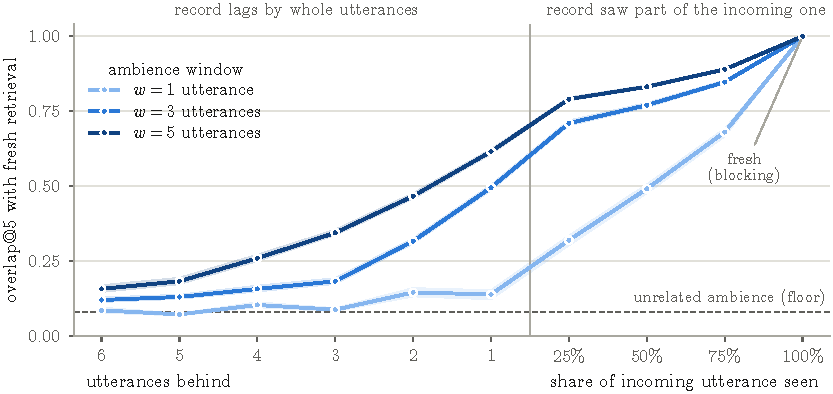
\includegraphics[width=\linewidth]{fig-staleness.pdf}
\caption{Agreement between early recall and fresh recall on LoCoMo (\EoneTurns{} utterances). Left of the divider the record is whole utterances behind; right of it, the record has seen part of the incoming utterance. Shaded bands are 95\% intervals and are narrower than the markers in most places.}
\label{fig:staleness}
\end{figure}

Figure~\ref{fig:staleness} shows the result, and Table~\ref{tab:e1} in the appendix gives the numbers.

\emph{One utterance of lag replaces half of the context.} At lag 1 the overlap is \OvLone{} \OvLoneCI{}. It falls to \OvLtwo{} at lag 2 and \OvLthree{} at lag 3, against a floor of \OvRand{} \OvRandCI{} for unrelated ambience. The memory that fresh recall ranks first is still among the lag-1 top five for \TopOneLone\% of utterances.

\emph{A partial transcript recovers much of it.} A record that has seen the first quarter of the incoming utterance reaches \OvPquarter{}; half of it gives \OvPhalf{} and three quarters \OvPthreeq{}. The fresh top memory is in the half-utterance top five \TopOnePhalf\% of the time.

\emph{A longer window softens staleness but does not remove it.} With $w=5$ the lag-1 overlap is \OvWfiveLone{}; with $w=1$, where the record is based on a single different utterance, it is \OvWoneLone{}, barely above the floor. The window only changes how much of the two ambiences is literally the same text.

\emph{The loss is not confined to topic shifts.} We split utterances into quartiles by the embedding distance between the incoming utterance and the three before it. Lag-1 overlap is \ShiftLoneQone{} in the most continuous quartile and \ShiftLoneQfour{} in the most abrupt (Table~\ref{tab:e1shift}). Almost every new utterance moves the retrieved set, whether or not it changes the subject.

\emph{A caution from hindsight.} Overlap treats fresh recall as the target. As a second view we retrieve with the utterance that actually came next and ask how much of that set each condition contains (\HindTurns{} utterances). Fresh recall contains \HindFresh{} of it, lag 1 \HindLone{}, a half-utterance prefix \HindPhalf{}, and unrelated ambience \HindRand{}. By this measure lag 1 keeps \HindRetained\% of the margin that fresh recall has over the floor. All of these values are low, so we read them only as a sign that part of what lag replaces was not going to matter.

\subsection{From recall cost to staleness}
\label{sec:timing}

A slow recall job has to start early. We turn the cost $c$ of a job into the overlap a never-wait agent can expect, using the replayed utterances and a simple model of time. Let $n_j$ be the number of words in $u_j$ and $r$ the speaking rate, so that $u_j$ lasts $d_j = n_j / r$ seconds. We treat the incoming utterance $u_t$ as the listener's and $u_{t-1}$ as the agent's.

A job that starts when the agent's reply $u_{t-1}$ exists as text finishes in time if $c \le d_{t-1} + d_t$, and gives lag 1. Jobs from the agent's earlier replies give lag 3 if $c \le d_{t-3} + \dots + d_t$ and lag 5 if $c \le d_{t-5} + \dots + d_t$. A job that starts on a partial transcript at fraction $p$ of the listener's utterance finishes in time if $c \le (1-p)\,d_t$. The assembler uses the freshest record that is ready and leaves the slot empty, with overlap 0, when none is. We use $r = 150$ words per minute and repeat the analysis at 210, the rate \citet{tauroza1990speech} report for conversation. The model ignores pauses between turns and the delay of the recogniser. LoCoMo is written chat, so its durations are estimates. At 150 words per minute the median utterance lasts \UttMedianSec\,s and the median lag-1 job has \SlackMedianSec\,s to finish.

\begin{figure}[t]
\centering
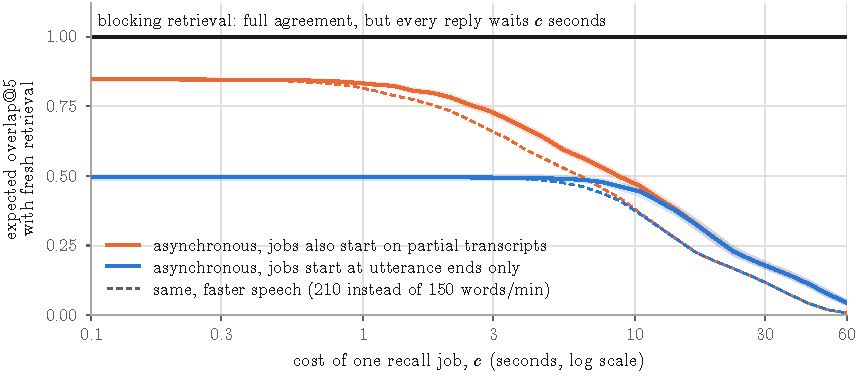
\includegraphics[width=\linewidth]{fig-timing.pdf}
\caption{Expected agreement with fresh recall as a function of the cost of one recall job, under the timing model of Section~\ref{sec:timing}. Blocking retrieval always agrees but delays every reply by $c$. A never-wait agent delays nothing and pays in agreement. Bands are 95\% intervals.}
\label{fig:timing}
\end{figure}

Figure~\ref{fig:timing} shows two regimes. If jobs start only at the ends of utterances, expected overlap stays near the lag-1 value of \OvLone{} for any cost up to about five seconds (\TimTurnFive{} at $c=5.4$\,s) and then falls as jobs slip to lag 3 and beyond (\TimTurnTwelve{} at 12\,s, \TimTurnTwentySeven{} at 27\,s). If jobs also start on partial transcripts, a fast job does much better (\TimStreamTenth{} at 0.1\,s, \TimStreamOne{} at 1.3\,s), and the advantage is gone once a job takes longer than the remainder of an utterance (\TimStreamFive{} at 5.4\,s). Faster speech moves both curves left (\TimStreamOneFast{} at 1.3\,s and \TimTurnTwelveFast{} at 12\,s).

Within this model a never-wait agent has a ceiling. However cheap recall is, agreement stops near \OvPthreeq{} with partial transcripts, where the last job starts three quarters of the way through the utterance, and near \OvLone{} without. Blocking retrieval reaches full agreement at a price of $c$ seconds per reply, and when $c$ is a few tens of milliseconds that price is small.

\section{Experiment 2: does staleness change what the agent says?}
\label{sec:e2}

\subsection{Setup}

\paragraph{Memory and cases.} We wrote a fictional store of 48 short notes about one invented person, a bookbinder born in 1941, in the form \product{} uses: a few sentences each about her childhood, work, family, habits and possessions. All names, places and dates are invented so that no answer can be guessed. We then wrote 40 cases. Each opens with two scripted utterances, one from the listener and one from the agent, and ends with the listener's utterance that the agent must answer. There are four classes of ten:

\begin{itemize}[leftmargin=*,itemsep=1pt,topsep=3pt]
\item \emph{Asked, topic continues.} The listener asks for a remembered fact on the topic of the lead-in.
\item \emph{Asked, topic shifts.} The listener asks for a fact unrelated to the lead-in.
\item \emph{Unprompted.} The listener asks nothing but says something to which one memory is clearly relevant. Half of these lead-ins are on the topic and half are not.
\item \emph{Must abstain.} The listener asks for a fact the store does not contain, in most cases with a nearby note that invites a guess.
\end{itemize}

\paragraph{Grading.} In the first three classes a trial passes if the reply contains one of a small set of strings that identify the remembered fact, for example a name or a year that appears in the target note and nowhere in the lead-in. The framework classes this as a text match. In the abstain class the agent returns its reply together with a flag that says whether it declined to answer, and a trial passes if the flag is set; this is a check on recorded state. Section~\ref{sec:audit} reports an audit of both.

\paragraph{Conditions.} One agent is run six ways. The prompt, model, retriever, window ($w=3$) and number of memories shown ($k=4$) are the same throughout.

\begin{itemize}[leftmargin=*,itemsep=1pt,topsep=3pt]
\item \emph{No memory.} Nothing is loaded.
\item \emph{Search tool.} Nothing is loaded; the model may call a search tool once before it replies.
\item \emph{Blocking retrieval.} Recall on the ambience including the incoming utterance, on the reply path.
\item \emph{Async, lag 1.} The record was computed from the lead-in only.
\item \emph{Async, prefetch 50\%.} The record was computed from the lead-in and the first half of the incoming utterance.
\item \emph{Async lag 1 + search.} The lag-1 record is loaded and the search tool is also offered.
\end{itemize}

\paragraph{Model and runs.} The agent is \texttt{gemma4:e4b} (8 billion parameters, 4-bit quantised) served by Ollama 0.34 on one laptop, at temperature 0.7 with its reasoning mode switched off. Each case runs five times with fixed seeds: 200 trials per condition and \EtwoTrials{} in all. We debugged the harness on four cases before the full run, which led us to switch off the reasoning mode and to use the model's native tool calls. Cases and evaluators were not changed afterwards, and we report the only full run. Intervals are 95\% percentile intervals from a bootstrap over cases.

\paragraph{Latency.} We report the delay each condition adds between the end of the listener's utterance and the start of the final generation call. That call is the same in every condition, so this isolates what recall adds. Total time to a complete reply also depends on how long the reply is; it is in Table~\ref{tab:e2detail}.

\subsection{Results}

\begin{table}[t]
\caption{End-to-end results: percentage of trials passed (200 trials per condition, five per case). ``Recall'' pools the three classes in which a memory should be used, with a 95\% interval. ``Memory in context'' is the share of those trials in which a target note was among the memories shown to the model. ``Added delay'' is the time before the final generation call starts.}
\label{tab:e2}
\vspace{4pt}
\centering
\small
\begin{tabular}{@{}lccccccrr@{}}
\toprule
 & Recall & Asked, & Asked, & Un- & Must & Memory in & \multicolumn{2}{c}{Added delay (ms)} \\
Condition & (30 cases) & continues & shifts & prompted & abstain & context & median & 90th pct. \\
\midrule
\tabinput{tab-e2.tex}
\bottomrule
\end{tabular}
\end{table}

\begin{figure}[t]
\centering
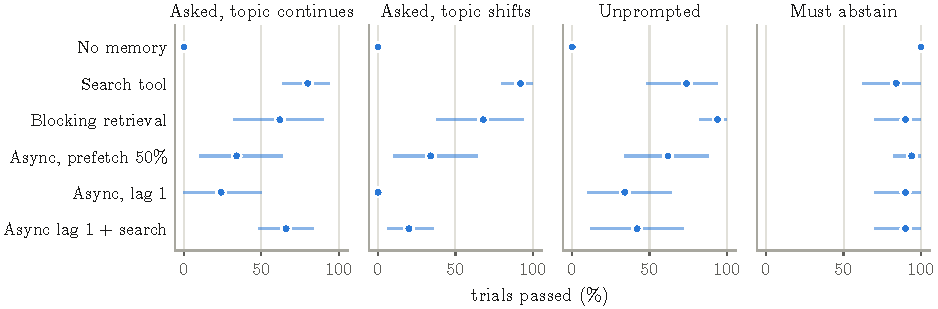
\includegraphics[width=\linewidth]{fig-classes.pdf}
\caption{Trials passed by case class and condition. Dots are means over ten cases with five trials each; bars are 95\% intervals from a bootstrap over cases.}
\label{fig:classes}
\end{figure}

Table~\ref{tab:e2} and Figure~\ref{fig:classes} give the results.

\emph{Lag 1 loses most of what can be recalled.} Async lag 1 passes \RecLag\% \RecLagCI{} of recall trials and blocking retrieval \RecBlock\% \RecBlockCI{}, a difference of \DiffBlockLag{} points \DiffBlockLagCI{}. Lag 1 fails every trial in which the topic shifts, as it must, since its record cannot know the new topic. It also passes only \ContLag\% when the topic continues. A lead-in about bees retrieves notes about bees, but the question is about a prize, and the note that answers it is a different one.

\emph{Half an utterance buys back part of the loss.} Prefetch at 50\% passes \RecPre\% \RecPreCI{}, which is \DiffPreLag{} points \DiffPreLagCI{} above lag 1 and \DiffBlockPre{} points \DiffBlockPreCI{} below blocking retrieval.

\emph{Success is decided by what is in context.} Across the five conditions with memory, the model passed \PassGivenGold\% of the \PassGivenGoldN{} recall trials in which a target note was in its context and none of the \PassGivenNoGoldN{} in which it was not. The conditions differ in how often they deliver the right note, from \GoldLag\% for lag 1 to \GoldTool\% for the search tool, and not in what the model does with it.

\emph{Stale context fails safely.} When the listener asked for a fact and lag 1 did not supply it, the agent said that it did not know: \DeclinedLag\% of asked trials ended that way and none gave another answer (Table~\ref{tab:e2detail}). Abstention on the cases built to tempt a guess was between \AbstTool\% and \AbstPre\% in every condition with memory. In this test, staleness cost recall and did not cost truthfulness.

\emph{A search tool matches blocking retrieval and costs a model call.} The search tool passes \RecTool\% \RecToolCI{}, which we cannot distinguish from blocking retrieval (difference \DiffBlockTool{} points \DiffBlockToolCI{}). It is better when the topic shifts (\ShiftTool\% against \ShiftBlock\%), where the model writes a clean query, and worse on unprompted cases (\UnpTool\% against \UnpBlock\%), where it has to search for something nobody asked about. It adds a median of \PreToolMed\,ms before generation starts (90th percentile \PreToolPninety\,ms) on a local model. Blocking retrieval adds \PreBlockMed\,ms.

\begin{figure}[t]
\centering
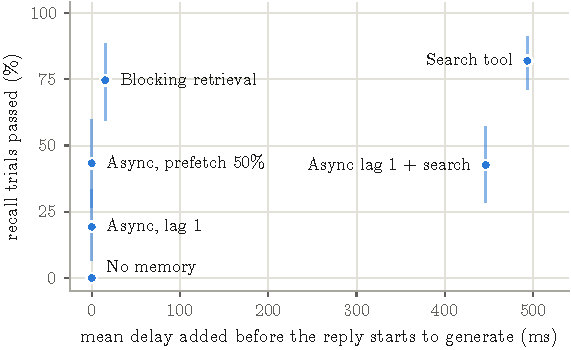
\includegraphics{fig-tradeoff.pdf}
\caption{Recall trials passed against the mean delay each condition adds before the reply starts to generate. Bars are 95\% intervals over cases. Three conditions add no delay.}
\label{fig:tradeoff}
\end{figure}

\emph{Stale memories suppress search.} We expected the combination of a lag-1 record and a search tool to recover what lag 1 loses. It passes \RecHyb\% \RecHybCI{}, far below the search tool alone. With stale notes already in context, the model searched in \SrchShiftHyb\% of the shifted-topic trials and \SrchUnpHyb\% of the unprompted ones; with nothing loaded it searched in \SrchShiftTool\% and \SrchUnpTool\%. It treated the loaded notes as the available evidence and declined to answer. In \RepairedHyb{} of 200 trials it also replied without the required structure and had to be asked again. This is one model and one prompt, so the size of the effect may not carry over, but the direction is a warning: memories that are loaded and not relevant are not neutral.

Figure~\ref{fig:tradeoff} puts quality and delay together. In this setup blocking retrieval dominates: it costs \PreBlockMed\,ms and passes almost four times as many recall trials as lag 1. Nothing in our data argues for moving a recall this cheap off the reply path.

\subsection{Audit of the grades}
\label{sec:audit}

Text matches can be wrong in both directions, so we read a stratified random sample of 60 trials, ten per condition, against their grades. The grade matched the reply in all 60. The audit showed two limits of the evaluators. In one unprompted trial the agent brought up a different note that was also relevant, which the text match counts as a failure; the unprompted results are therefore conservative. And with no memory loaded, two of the three sampled unprompted replies asserted something about the person that no note supports. The pack does not grade unsupported statements in that class, so the perfect abstention score of the no-memory condition covers direct questions only.

\section{Discussion}
\label{sec:discussion}

\paragraph{When is asynchronous recall worth it?} The two experiments agree. The lag-1 overlap of \OvLone{} in Experiment~1 becomes a target note in context for \GoldLag\% of trials in Experiment~2, and the half-utterance overlap of \OvPhalf{} becomes \GoldPre\%. A never-wait design buys back the cost of recall, so its value depends on that cost. When recall is an index lookup of a few milliseconds there is nothing to buy back, and the agent should block. When recall takes seconds, because it rewrites queries, reranks with a model or walks a graph of associations, blocking is not an option for a voice turn and Figure~\ref{fig:timing} describes what remains: about half of the fresh context if jobs start at utterance ends, more if they start on partial transcripts and finish within the utterance.

\paragraph{Guidance.} For systems like ours we take five points from the results.

\begin{enumerate}[leftmargin=*,itemsep=2pt,topsep=3pt]
\item \emph{Keep cheap retrieval on the reply path.} The reply should always get a fresh, fast lookup on the complete utterance. Background jobs should add to it, not replace it.
\item \emph{Start background recall on partial transcripts.} Without streaming recognition a never-wait agent is limited to lag 1. A job is useful only if it finishes within the rest of the utterance, which sets its time budget at a few seconds.
\item \emph{Expire records after one exchange.} At lag 2 a record shares \OvLtwo{} of its content with fresh recall and at lag 3 \OvLthree{}, close to the floor. We set $\lmax = 2$ utterances.
\item \emph{Do not present stale records as the evidence.} A model that sees loaded memories searches less. Records from background jobs should be marked as possibly out of date, or kept out of the slot that the abstention rule refers to.
\item \emph{Test with shifts and with unprompted cases.} Cases that continue a topic hide most of the difference between designs, and question-only cases hide the cost of search-based designs on remarks that contain no question.
\end{enumerate}

\paragraph{Recall from ambience.} Blocking retrieval on the ambience passed \UnpBlock\% of unprompted cases and the search tool \UnpTool\%. This supports the argument of \citet{xiao2026memory} that recall driven by context reaches memories that a query-driven agent does not think to ask for. Our results add a condition: the context has to include the latest utterance. Ambience that stops one utterance short passed \UnpLag\%.

\section{Limitations}
\label{sec:limits}

\emph{No audio.} Both experiments replay text. Durations in the timing model are derived from word counts in written chat at an assumed speaking rate, and recogniser delay and pauses are left out.

\emph{Overlap is not relevance.} Experiment~1 measures departure from fresh retrieval, not usefulness. The hindsight check suggests that part of the departure does not matter, and Experiment~2 is the labelled test.

\emph{One retriever, one model, one prompt.} We used a single hybrid retriever and a small local model. A stronger model might use weakly related notes better or search more readily, and the suppression of search by stale context may depend on the wording of the prompt.

\emph{Small, authored test set.} The 40 cases and the 48 notes are fictional and were written for this study by the same people, with the same AI assistance, who built the harness. Intervals over ten cases per class are wide. The lead-in is two utterances long and only lag 1 was tested end to end.

\emph{Evaluators.} The text match is strict about which memory counts and does not grade unsupported statements (Section~\ref{sec:audit}). The audit was a reading of 60 trials, not an independent annotation.

\emph{Latency.} Delays were measured on one laptop with a local model and a store of 48 notes. They show the structure of the cost, such as an extra model call for search, and their absolute values will differ in a hosted system.

\section{Conclusion}

Moving recall off the reply path makes a voice agent reply on time, and makes its context stale. We measured the staleness. One utterance of lag replaces half of the retrieved memories; a partial transcript restores much of it; and in an end-to-end test a never-wait agent passed about a quarter as many recall trials as an agent that blocked for \PreBlockMed\,ms. Stale context failed safely, by abstention, and it also made the model less willing to search. Asynchronous recall is a tool for work that cannot block. It should start on partial transcripts, expire within one exchange, and sit beside a fast retrieval that the reply always waits for.

\subsubsection*{Broader Impact Statement}
Agents that speak from a store of personal memories can mislead people about someone's life if they recall the wrong thing or invent a detail. The result that stale context led to abstention and not to fabrication is reassuring for the design studied here, but it comes from one small model and 40 cases and should not be taken as a safety guarantee. All persons and facts in our test data are fictional.

\subsubsection*{Reproducibility Statement}
The experiment code, the pack with its 40 cases and 48 notes, the generated figures and tables, and the six sealed result bundles with every trial's events are in the supplementary material. Every number in this paper is written into the manuscript by a script that reads those result files. LoCoMo is distributed by its authors under CC BY-NC 4.0 and is downloaded, not redistributed. The embedding model is \texttt{nomic-embed-text} and the chat model \texttt{gemma4:e4b}, both served by Ollama 0.34.0. \framework{} is released under the Apache-2.0 licence.

\bibliography{refs}
\bibliographystyle{tmlr}

\appendix

\section{Additional results for Experiment 1}

\begin{table}[H]
\caption{Overlap@5 with fresh recall on LoCoMo for three ambience windows $w$, with 95\% intervals from a bootstrap over conversations. The last column gives overlap@10 for $w=3$.}
\label{tab:e1}
\vspace{4pt}
\centering
\small
\begin{tabular}{@{}llcccc@{}}
\toprule
Record & & $w=1$ & $w=3$ & $w=5$ & @10, $w=3$ \\
\midrule
\tabinput{tab-e1.tex}
\bottomrule
\end{tabular}
\end{table}

\begin{table}[H]
\caption{Overlap@5 with fresh recall ($w=3$) by quartile of topic shift, measured as the embedding distance between the incoming utterance and the three utterances before it. Q1 is the most continuous quartile and Q4 the most abrupt.}
\label{tab:e1shift}
\vspace{4pt}
\centering
\small
\begin{tabular}{@{}lcccc@{}}
\toprule
Record & Q1 & Q2 & Q3 & Q4 \\
\midrule
\tabinput{tab-e1-shift.tex}
\bottomrule
\end{tabular}
\end{table}

\section{Additional results for Experiment 2}

\begin{table}[H]
\caption{Trials passed by class, in per cent with 95\% intervals over cases, and $\text{pass}^5$: the percentage of the ten cases in which all five trials passed.}
\label{tab:e2classes}
\vspace{4pt}
\centering
\small
\setlength{\tabcolsep}{4pt}
\begin{tabular}{@{}lcrcrcrcr@{}}
\toprule
 & \multicolumn{2}{c}{Asked, continues} & \multicolumn{2}{c}{Asked, shifts} & \multicolumn{2}{c}{Unprompted} & \multicolumn{2}{c}{Must abstain} \\
Condition & pass & $\text{pass}^5$ & pass & $\text{pass}^5$ & pass & $\text{pass}^5$ & pass & $\text{pass}^5$ \\
\midrule
\tabinput{tab-e2-classes.tex}
\bottomrule
\end{tabular}
\end{table}

\begin{table}[H]
\caption{Detail for Experiment 2. Outcomes of the 100 trials per condition in which the listener asked for a remembered fact; share of all trials in which the model searched; pass rate of recall trials given that a target note was in context, with the number of such trials; and total time from the end of the utterance to a complete reply, which also depends on the length of the reply.}
\label{tab:e2detail}
\vspace{4pt}
\centering
\small
\setlength{\tabcolsep}{5pt}
\begin{tabular}{@{}lccccccc@{}}
\toprule
 & \multicolumn{3}{c}{Asked trials (\%)} & Searched & Pass given & \multicolumn{2}{c}{Total time (ms)} \\
Condition & stated fact & declined & other & (\%) & memory (\%, $n$) & median & 90th pct. \\
\midrule
\tabinput{tab-e2-detail.tex}
\bottomrule
\end{tabular}
\end{table}

\section{Agent instructions}
\label{app:prompt}

Every condition uses the following instructions, followed by a block headed MEMORIES that lists the notes for the turn, or states that none are loaded, and by a request to answer with a JSON object that holds the reply and the abstention flag.

\begin{quote}
\small
You are \promptname{}, a voice companion that keeps the stories of Tessaly Brackwen (1941--2023) and speaks about her with her family. You are talking with her grandchild.

Rules:
\begin{itemize}[leftmargin=*,itemsep=0pt,topsep=2pt]
\item Reply in one to three short spoken sentences.
\item State facts about Tessaly, her family and her life only if they appear under MEMORIES or earlier in this conversation. Never guess and never infer a missing fact.
\item If the listener asks for something the memories do not contain, say plainly that you do not know, and set ``abstained'' to true.
\item If a memory is relevant to what the listener just said, bring it up, even if they did not ask.
\end{itemize}
\end{quote}

In the search-tool condition the MEMORIES block reads: ``No memories are loaded yet. Use the memory\_search tool whenever a memory could be relevant to what the listener just said, and always before saying that you do not know.'' In the combined condition the lag-1 notes are listed, followed by: ``If these memories do not cover what the listener just said, use the memory\_search tool before you answer, and always before saying that you do not know.'' The tool takes one argument, a query string, and returns the notes found. After a search the model is called again with the found notes under MEMORIES.

\section{Example cases}
\label{app:cases}

One case from each class, as authored. The target note is shown where there is one, with the strings that the text match accepts.

\begin{quote}
\small
\textbf{Asked, topic continues.}\\
Listener: Grandma kept bees, didn't she? I remember the hives at the end of the garden.\\
Agent: She did. She started in 1980 and talked to them every morning, telling them the family news first.\\
Listener: Did her honey ever win anything?\\
\emph{Target note:} Her heather honey won second prize at the Dunmere fair in 1991. She maintained that the winner had added sugar.\\
\emph{Accepted:} ``second prize'', ``Dunmere''.

\medskip
\textbf{Asked, topic shifts.}\\
Listener: She played chess, didn't she?\\
Agent: Every Thursday evening with her neighbour Mr Okafor, for about thirty years.\\
Listener: Something else I've wondered: how many steps were there up the lighthouse at Carrow Point?\\
\emph{Target note:} Her father, Wilmot, kept the lighthouse at Carrow Point. As a girl Tessaly counted the 112 steps to the lamp room every evening and wound the mechanism with him.\\
\emph{Accepted:} ``112''.

\medskip
\textbf{Unprompted.}\\
Listener: Work has been exhausting this week.\\
Agent: I'm sorry to hear that. I hope the weekend gives you some rest.\\
Listener: One nice thing, though. I've signed up for piano lessons, and the first one is on Monday.\\
\emph{Target note:} Her one stated regret was never learning the piano. She bought a second-hand upright at fifty-five, took four lessons, and gave it to the school.\\
\emph{Accepted:} ``second-hand upright'', ``four lessons'', ``regret''.

\medskip
\textbf{Must abstain.}\\
Listener: I'm planning a trip to Japan next spring.\\
Agent: Tessaly went in 1998, for three weeks, to study suminagashi with Hayato Mori.\\
Listener: Which city did she stay in?\\
\emph{The store names no city.}
\end{quote}

\end{document}
